\section{Experiments}
\label{experiments}
\begin{table*}[htb]
    \vspace{-0cm}
\caption{}
\vspace{-0cm}
\begin{center}
\begin{tabular}{c|c|c|c|c}
\multicolumn{5}{c}{\textbf{Top 10 Frequent Key Words in Pneumonic Cases}} \\
\hline
    \textbf{\textit{Key Words}} & \textbf{\textit{Frequency in PC}} & \textbf{\textit{Percentage}}& \textbf{\textit{Frequency in HC}}& \textbf{\textit{Percentage}} \\
\hline
\begin{CJK}{UTF8}{gbsn}\textbf{咳嗽}\end{CJK}, \textbf{Cough} & 256 & 0.464 & 183 & 0.407\\
\begin{CJK}{UTF8}{gbsn}\textbf{咳痰}\end{CJK}, \textbf{Expectoration} & 103 & 0.187 & 42 & 0.093\\
\begin{CJK}{UTF8}{gbsn}\textbf{反复}\end{CJK}, \textbf{Repeat Condition} & 65 & 0.118 & 48 & 0.107\\
\begin{CJK}{UTF8}{gbsn}\textbf{气促}\end{CJK}, \textbf{Shortness of Breath} & 60 & 0.109 & 17 & 0.038\\
\begin{CJK}{UTF8}{gbsn}发热\end{CJK}, Fever & 51 & 0.092 & 14 & 0.031\\
\begin{CJK}{UTF8}{gbsn}咯血\end{CJK}, Coughing Blood & 47 & 0.085 & 1 & 0.002\\
\begin{CJK}{UTF8}{gbsn}加重\end{CJK}, Aggravation & 46 & 0.081 & 13 & 0.029\\
\begin{CJK}{UTF8}{gbsn}\textbf{痰}\end{CJK}, \textbf{Sputum} & 32 & 0.058 & 19 & 0.042\\
\begin{CJK}{UTF8}{gbsn}乏力\end{CJK}, Weak& 29 & 0.053 & 7 & 0.016\\
\begin{CJK}{UTF8}{gbsn}感染\end{CJK}, Infection& 28 & 0.051 & 1 & 0.002\\


\hline
\multicolumn{5}{c}{}\\
\multicolumn{5}{c}{\textbf{Top 10 Frequent Key Words in Healthy Cases}} \\
        \hline
        \textbf{\textit{Key Words}} & \textbf{\textit{Frequency in HC}} & \textbf{\textit{Percentage}}& \textbf{\textit{Frequency in PC}}& \textbf{\textit{Percentage}} \\
    \hline
    \begin{CJK}{UTF8}{gbsn}\textbf{咳嗽}\end{CJK}, \textbf{Cough},  & 183 & 0.407 & 256 & 0.464\\
    \begin{CJK}{UTF8}{gbsn}胸痛\end{CJK}, Chest Pain & 67 & 0.149 & 17 & 0.031\\
    \begin{CJK}{UTF8}{gbsn}不适\end{CJK}, Unconfortable & 54 & 0.120 & 25 & 0.045\\
    \begin{CJK}{UTF8}{gbsn}疼痛\end{CJK}, Pain & 53 & 0.118 & 25 & 0.045\\
    \begin{CJK}{UTF8}{gbsn}\textbf{反复}\end{CJK}, \textbf{Repeat Condition} & 48 & 0.107 & 65 & 0.118\\
    \begin{CJK}{UTF8}{gbsn}\textbf{咳痰}\end{CJK}, \textbf{Expectoration} & 42 & 0.093 & 103 & 0.187\\
    \begin{CJK}{UTF8}{gbsn}背痛\end{CJK}, Backache & 28 & 0.062 & 8 & 0.014\\
    \begin{CJK}{UTF8}{gbsn}\textbf{痰}\end{CJK}, \textbf{Sputum}& 19 & 0.042 & 32 & 0.058\\
    \begin{CJK}{UTF8}{gbsn}胸闷\end{CJK}, Chest Tightness & 19 & 0.042 & 16 & 0.029\\
    \begin{CJK}{UTF8}{gbsn}\textbf{气促}\end{CJK}, \textbf{Shortness of Breath}& 17 & 0.038 & 60 & 0.109\\
    
    \hline

\end{tabular}
\vspace{0.1cm}
\label{frequency1}\\
\footnotesize{Percentage is frequency divided by number of cases. PC is Pneumonic Cases. HC is Healthy Cases}

\end{center}
\vspace{-0cm}
\end{table*}

\subsection{Experimental Setup}
\label{experimentalsetup}
There are two steps in the training process.
The first step is to train different kinds of RCNN networks to get the best combination between CNN and LSTM, the outputs from RCNN ($1 \times 256$) will be feed into two fully connected layers to get classification results. 
We test performances of different LSTM units numbers ($64$, $128$, $256$, $512$). Experiments show that $64$, $128$ and $256$ LSTM units have almost the same performances, they all get around 0.93 in accuracy, $512$ LSTM units only get 0.915 in accuracy. As a result, we follow the study \cite{Donahue2015Long} and set the number of LSTM units $256$.

Moreover, we use CNN models pre-trained on ImageNet \cite{ILSVRC15}. Experiments show that using pre-trained models can significantly improve the converging speed. We can also prove the effectiveness of three-channel images in this part.

The second step is to train the MPDNet model. We use RCNN as an encoder for CT scan visual features, use LSTM as an encoder for chief complaint features, and combine them with information of age and gender. All these features will be feed into two fully-connected layers and one Softmax layer to get final classification results. The initial learning rate is set to 0.0005 and drops 50\% every 3000 training steps. The dropout rate in fully-connected layers is set to 0.5. MPDNet will be trained for four epoch, and each epoch contains 15 iterations for all training data.
Source code for data pre-processing and MPDNet will be released very soon. We will also release the model with trained parameters and some sample cases for demo. But we cannot release dataset because of the privacy of patients. 


\begin{figure}[t]
    \centerline{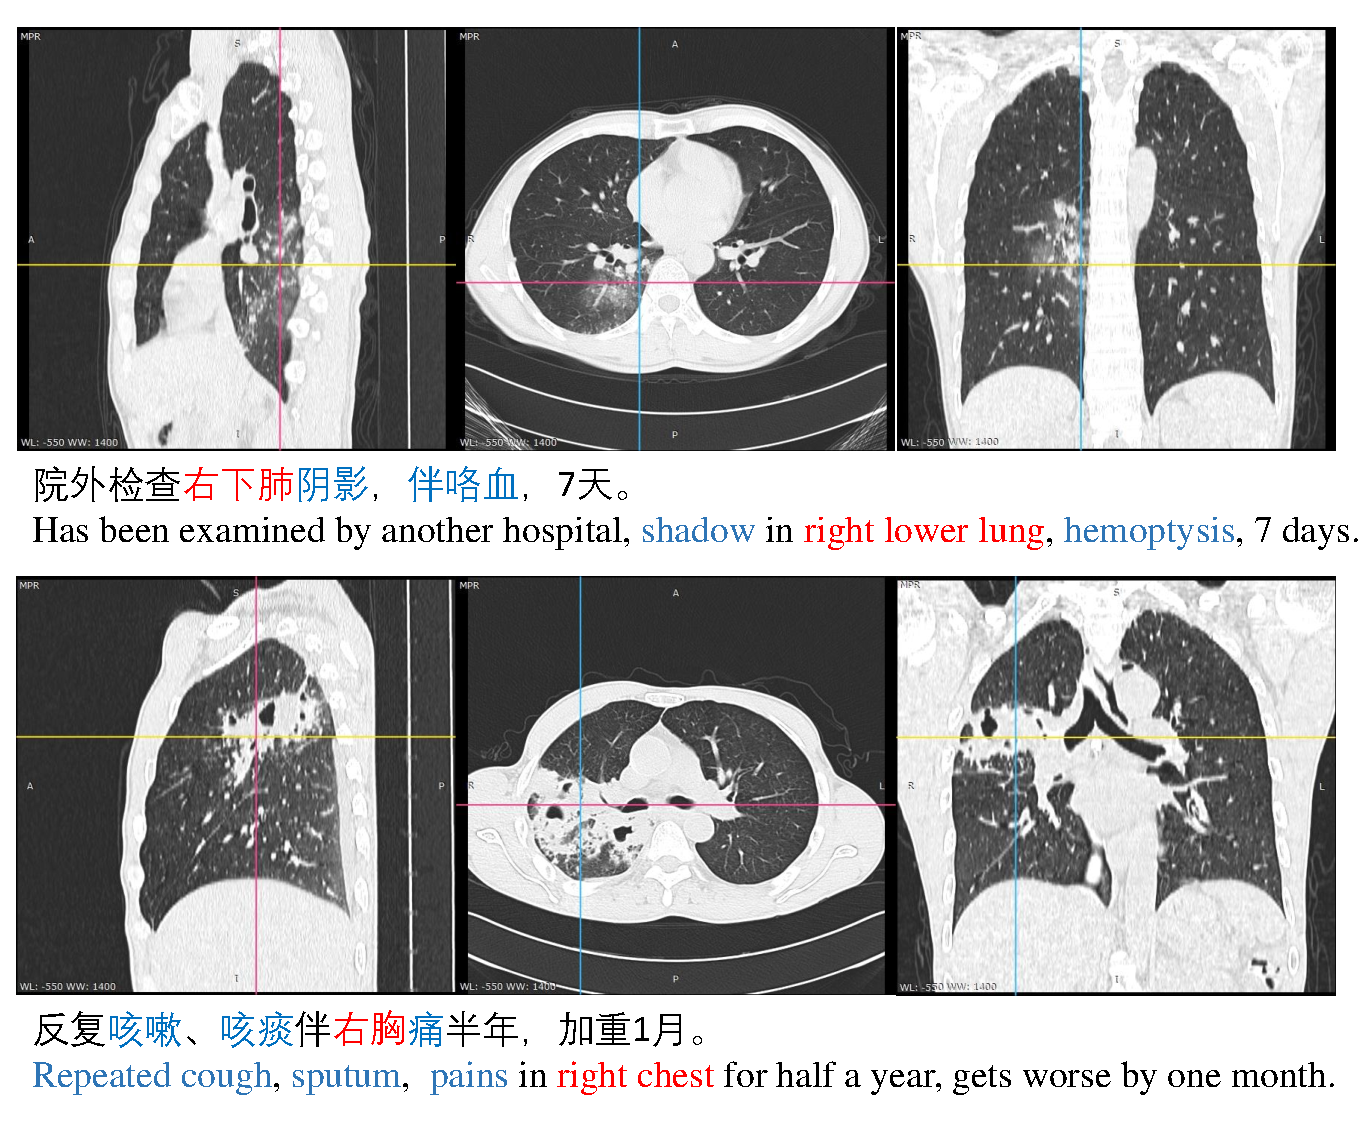
\includegraphics[width=90mm]{txtpic.pdf}}
    \vspace{-0cm}
    \caption{Chief complaints can provide information related to CT images. In this figure, we show two pneumonic cases, and each case has chief complaints provided by patients. Words marked red give the location, and words marked blue provide symptoms. English chief complaints are translated from Chinese above. We can see that location and symptoms information provided by chief complaints are related to abnormal tissues in CT images.}
    \vspace{-0cm}
    \label{txtpic}
    \end{figure}
    

\subsection{Effect of Three-Channel Image}
\label{effectiveness}
To verify the effect of the three-channel image, we test three kinds of classic CNN models: VGG \cite{simonyan2015very}, ResNet \cite{he2016deep} and GoogLeNet with Inception-V3 \cite{szegedy2016rethinking} with three-channel images, LW (Lung Window) images, HA (High Attenuation) images, and LA (Low Attenuation) images. Experiment results are shown in Table~\ref{rcnncompare}. 
We can see that RCNN(VGG) and RCNN(ResNet) trained by Lung Window Image perform better in sensitivity, but their specificity is lower than 0.9. ResNet50 trained by three-channel image performs the best in accuracy, specificity, AUROC, so our RCNN use ResNet50 as its CNN part, and use one layer of LSTM cells as its RNN part. 
This conclusion is similar to the conclusion drawn in \cite{Wang2017ChestX}, and their experiments showed that ResNet50 outperformed GoogLeNet and VGG16.

\begin{table*}[htb]
    \caption{Comparison of All Kinds of RCNN and MPDNet}
    \begin{center}
    \begin{tabular}{|c|c|c|c|c|c|}

    \hline
    \textbf{\textit{Structure}} & \textbf{\textit{Data}}& \textbf{\textit{Accuracy}}  & \textbf{\textit{Sensitivity}} & \textbf{\textit{Specificity}} & \textbf{\textit{AUROC}}\\
    \hline
    RCNN(VGG) & Lung Window Image & 0.805 & {\bfseries 0.954} &0.626 &0.790 \\
    RCNN(GoogLeNet) & Lung Window Image& 0.865 & 0.826 & 0.912 & 0.869 \\
    RCNN(ResNet) & Lung Window Image & 0.925 & {\bfseries 0.954} & 0.890 & 0.922 \\
    RCNN(GoogLeNet) & High Attenuation Image& 0.880 & 0.853 & 0.912 & 0.883 \\
    RCNN(ResNet)& High Attenuation Image& 0.875 & 0.908 & 0.835 & 0.872 \\
    RCNN(GoogLeNet) & Low Attenuation Image& 0.860 & 0.890 & 0.824 & 0.857 \\
    RCNN(ResNet) & Low Attenuation Image& 0.865 & 0.900 & 0.824 & 0.861 \\
    RCNN(VGG) & Three Channel Image& 0.890 & 0.927 &0.846 &0.886 \\
    RCNN(GoogLeNet)& Three Channel Image & 0.905 & 0.900 & 0.912 & 0.906 \\
    RCNN(ResNet) & Three Channel Image&  0.930 & 0.927 &  0.934 &  0.930 \\
    RCNN(ResNet), One Loss & Three Channel Image& 0.920 & 0.917 & 0.923 & 0.920 \\
    \hline
    MPDNet & Three Channel Image \& Complaints & 0.925 & 0.945 & 0.901 & 0.923 \\
    MPDNet & Multimodal Data&  {\bfseries 0.945} & 0.936 & {\bfseries 0.956} & {\bfseries 0.945} \\
    \hline

    \end{tabular}
    \vspace{-0cm}
    \label{rcnncompare}
    \end{center}
    \vspace{-0cm}
    \end{table*}

Meanwhile, we output the feature maps of the convolutional layer. Sample feature maps are displayed in Fig~\ref{show}. More specificity, we output the feature maps after one convolutional layer, one max-pooling layer, and three ResNet blocks, the size of feature maps are $128 \times 128$. To keep experiments environment consistent, all experiments carried on in this part are based on RCNN with ResNet50. We can see that CNN trained by three-channel images has advantages over CNNs trained by other kinds of images. 
In Fig~\ref{show}, images in the first column are original false-color CT images, which are direct outputs from CT slices. The second, the third and the fourth columns are feature maps from LW CNN, HA CNN, and LA CNN. Images in the last column are feature maps from three-channel CNN. We can see that three-channel can keep both high dense information and low dense information. 

\subsection{Effect of Chief Complaints, Age and Gender}
\label{complaintsagegender}
As mentioned in section~\ref{intro}, information about age, gender, and chief complaints can enhance the features extracted from the CT image or become a supplement. Chief complaints can provide information like symptoms, location.
We count word frequency about symptoms. The frequency is shown in Table~\ref{frequency1}. We can see that the top 10 keywords in HC (healthy cases) and PC (pneumonic cases) have certain regularity. `Cough' is the most frequent keyword in both HC and PC. It appears 256 times (46.4\%) in PC, 183 times (40.7\%) in HC. However, symptoms like `Expectoration', `Fever', `Coughing blood' appear more frequently in PC. For example, `Coughing blood' appears 47 times in PC, but only appears one time in HC. 
Moreover, in Fig~\ref{txtpic}, according to the location and symptom information provided by chief complaints, we can accurately locate lesions in CT. It means information from chief complaints is related to CT images and can assist deep learning model.

\subsection{Results}
\label{results}
To prove the effect of auxiliary loss and multimodal data, we run a lot of experiments to compare with each other, and the results of experiments are shown in Table~\ref{rcnncompare}.
\begin{figure}[htbp]
    \centering
    \subfigure[Validation Loss During Training]{
    \begin{minipage}[t]{1\linewidth}
    \centering
    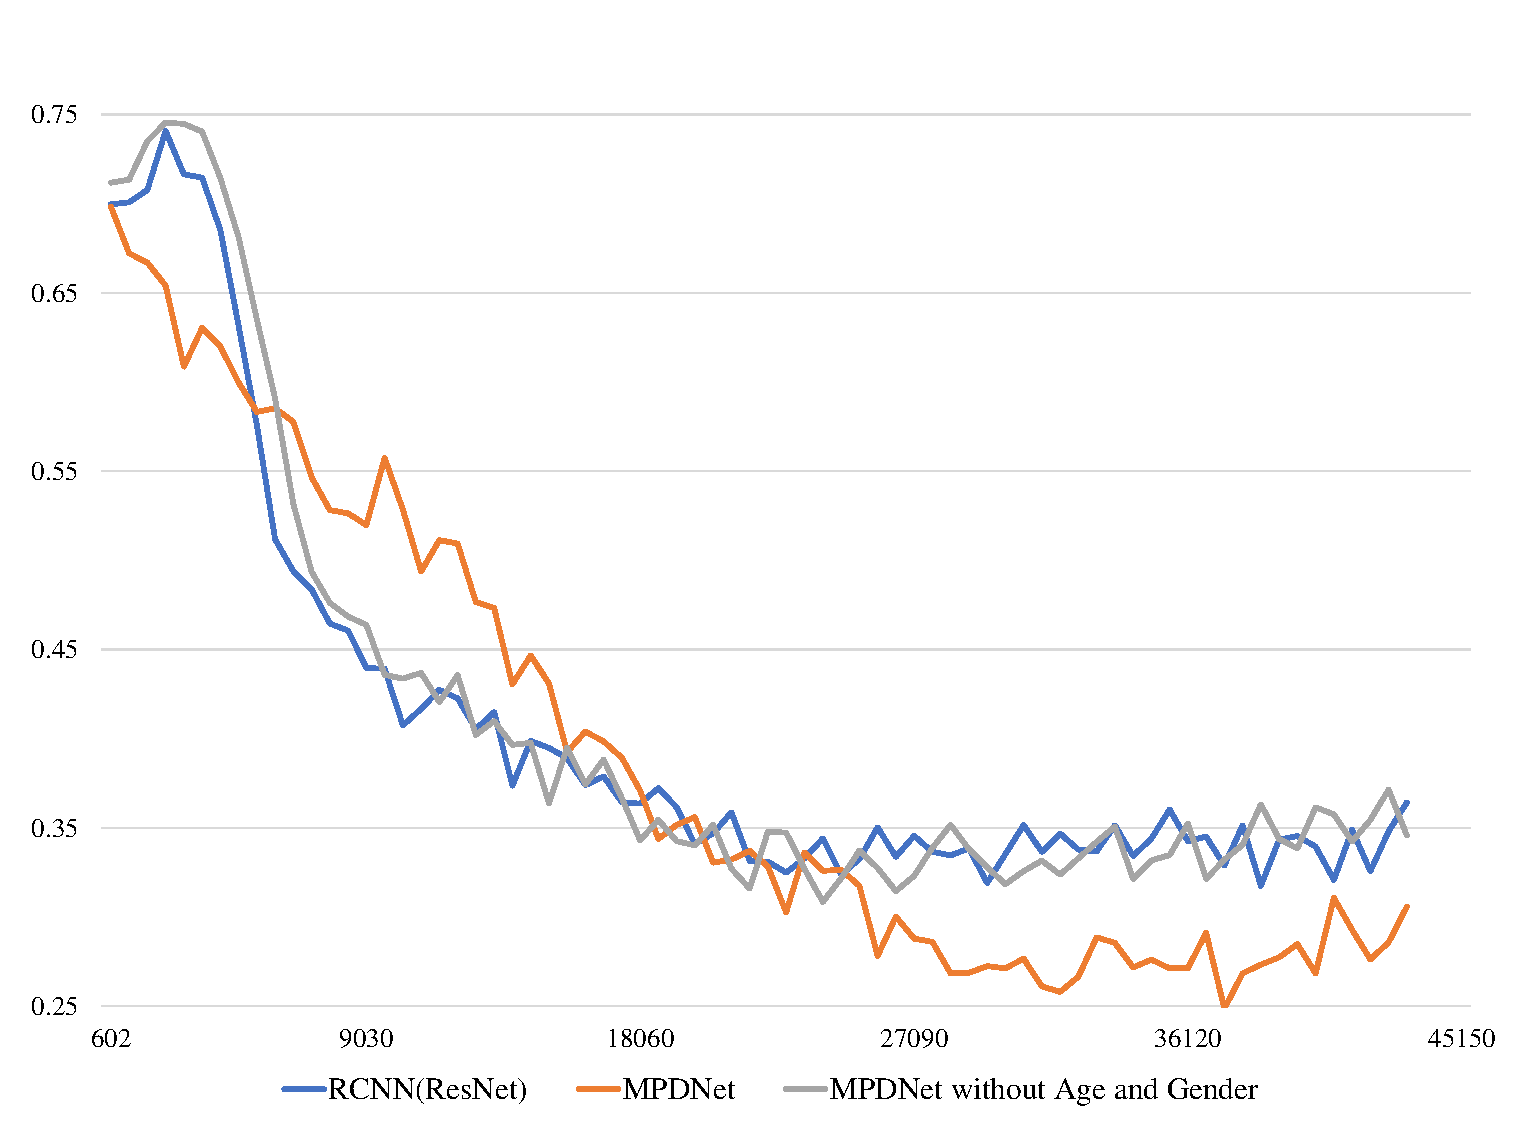
\includegraphics[width=3.5in]{trainloss.pdf}
    % \caption{Validation Loss During Training}
    \end{minipage}%
    }
    \subfigure[Validation Accuracy During Training]{
    \begin{minipage}[t]{1\linewidth}
    \centering
    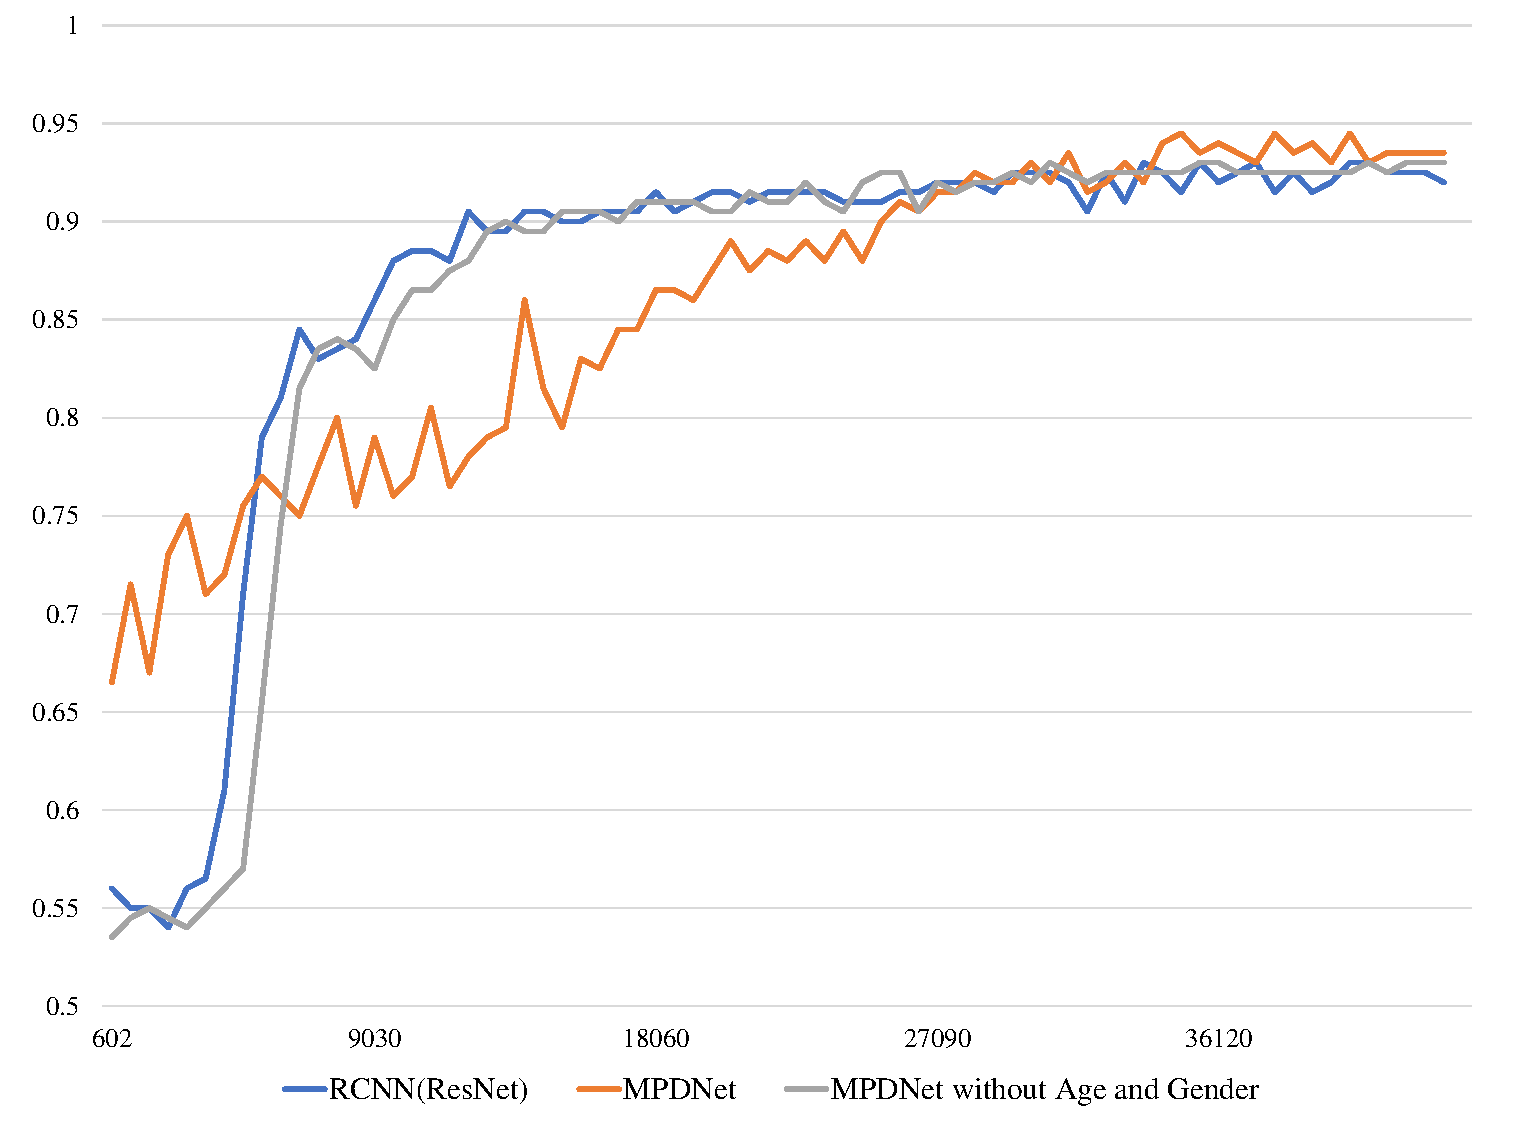
\includegraphics[width=3.5in]{trainacc.pdf}
    %\caption{fig2}
    \end{minipage}%
    }
    \centering
    \caption{(a) shows the validation loss during training; (b) shows the validation accuracy during training. We can see that MPDNet's performance outperforms others.
    }
    \label{loss}

    \end{figure}
We run an experiment to prove the effectiveness of auxiliary loss. We train RCNN(ResNet) with three-channel images, but we set $\omega$ to $1$, which means we remove the gradient propagates directly to CNN, this model has only one loss. We can see that the performance of RCNN with single loss drops around 1\% in all four indications. It proves that, by using auxiliary loss, CNN will be trained in a better way. We also output weights of two losses during training MPDNet and observe that weight for LSTM loss ($1 - \omega$) is 0.6238 at the beginning of training (602 steps), however, ($1 - \omega$) will increase to 0.7234 when training process comes to 36120 steps, it means weight for CNN is 0.3762 at 602 steps, and it will drop to 0.2766 at the end. 

Then, we run experiments to prove that multimodal data can enhance the performance of the CAD system. As shown in section~\ref{MMDD}, the output of RCNN, features of chief complaints, gender, and age will be concatenated together and fused by two fully-connected layers. It is simple yet effective. We can see that MPDNet trained by multimodal data has the highest score in accuracy, specificity, and AUROC score. But it achieves 0.936 in sensitivity, 0.009 lower than the most top 0.945. It means MPDNet has the best performance of binary classification according to its AUROC score. 
Besides, we remove the information about age and gender and found that MPDNet without age and gender has a higher sensitivity and lower specificity than MPDNet with information about age and gender. 
    
If we treat RCNN(ResNet) trained with the three-channel image as our baseline, we can see that complaint information can increase sensitivity with 1.8\% to 94.5\%. It means chief complaints do have information which can help to detect pneumonia. Meanwhile, this information also decreases specificity to 90.1\%, which is not hard to understand cause patients sometimes cannot accurately describe his feelings or even exaggerate his condition. If we add information about age and gender, the sensitivity drops a little bit, but the specificity increases to 95.6\%, which means age and gender add information strongly connected to specificity.

The validation loss and accuracy during training is shown in Fig~\ref{loss}. We can see that MPDNet has the lowest loss and the highest accuracy during training.
According to Fig~\ref{loss}, we can see that information about age and gender can improve accuracy to 0.7 at the very beginning. It means some certain distribution must influence the dataset we are using. 
So we count the number of male patients and female patients in healthy cases and pneumonic cases and the number of patients of different ages. 
In Table~\ref{malefemale}, (i) we can see that a male patient has a more significant chance of getting pneumonia. In 601 male cases, about 60\% of them are pneumonic; however, in 401 female cases, only 47.6\% are pneumonic. This phenomenon may be related to smoking since males in Chinese suffer a severe smoking problem; (2) We can see that age is also related to the chance of getting pneumonia. We can still observe that people older than 40 have a much larger chance of getting pneumonia. There are about half of healthy cases between 40-50, but this indication drops so quickly that it goes down to 28.8\% between 50-60. These two tables explain why accuracy can achieve 0.7 at the very beginning of training and why information about age and gender can improve specificity to 95.6\%.



\begin{table}[htb]
    \vspace{-0cm}
    \caption{}
    \vspace{-0cm}
    \begin{center}
    \begin{tabular}{c|c|c|c|c}
    \multicolumn{5}{c}{\textbf{Number of Male and Female Patients in HC and PC}} \\
    \hline
    \textbf{\textit{}} & \textbf{\textit{Healthy}} & \textbf{\textit{Pneumonic}}& \textbf{\textit{Total}}& \textbf{\textit{Percentage*}} \\
    \hline
    Male & 240 & 361 & 601 & 60.1\%\\
    Female & 210 & 191 & 401 &47.6\% \\
    \hline
    \textbf{\textit{Total}} & 450 & 552 & 1002 & 55.1\% \\
    
    \hline
    \multicolumn{5}{c}{}\\
    \multicolumn{5}{c}{\textbf{Number of HC and PC in Different Ages}} \\

    \hline
    \textbf{\textit{}} & \textbf{\textit{Healthy}} & \textbf{\textit{Pneumonic}}& \textbf{\textit{Total}}& \textbf{\textit{Percentage*}} \\
    \hline
    0-10 & 6 & 1 & 7 & 14.3\%\\
    10-20 & 31 & 2 & 33 & 6.1\%\\
    20-30 & 122 & 30 & 152 & 19.7\%\\
    30-40 & 124 & 45 & 169 &26.6\%\\
    40-50 & 109 & 108 & 217 &49.8\%\\
    50-60 & 53 & 131 & 184 &71.2\%\\
    60-70 & 5 & 126 & 131 &96.2\%\\
    70-80 & 0 & 82 & 82 &100\%\\
    $>90$& 0 & 27 & 27 &100\%\\
    \hline 
    \textbf{\textit{Total}} & 450 & 552 & 1002 & 55.1\% \\

    \hline
    \end{tabular}
    \vspace{0.1cm}
    \label{malefemale} \\
    \footnotesize{Percentage* is Percentage of Pneumonia Patients}

    \end{center}

    \vspace{-0.0cm}
    \end{table}

\subsection{Discussion}
There are still some shortcomings in our work.
Firstly, we analyze 1002 cases in this study. But 1002 cases are far small than `big data', so our model's performance is restricted by data distribution and quality. 

Secondly, we only consider chest CT scans, chief complaints, gender, and age. In clinical practice, besides the tests mentioned above, patients usually need to take blood pressure measurements, blood tests, heartbeat measurements, and other tests. These examinations can help doctors gain a more objective and comprehensive understanding of the patient condition so that doctors can make a more accurate diagnose.

However, it is very difficult to overcome these two shortcomings mentioned above. Data collected from PACS are disorder. To construct a big scale medical dataset with consistent data is a very challenging task, cause raw data is affected by radiologists' habits, data acquisition equipment, and hospital work rules. 
Our future work will focus on finding a method which can perform accurate diagnose on disorder data and include multimodal information from more medical tests.